

% This document was generated by the publish-function
% from GNU Octave 10.1.0



\documentclass[10pt]{article}
\usepackage{listings}
\usepackage{mathtools}
\usepackage{amssymb}
\usepackage{graphicx}
\usepackage{hyperref}
\usepackage{xcolor}
\usepackage{titlesec}
\usepackage[utf8]{inputenc}
\usepackage[T1]{fontenc}
\usepackage{lmodern}


\lstset{
language=Octave,
numbers=none,
frame=single,
tabsize=2,
showstringspaces=false,
breaklines=true,
inputencoding=utf8,
extendedchars=true,
literate=
  {á}{{\'a}}1 {é}{{\'e}}1 {í}{{\'i}}1 {ó}{{\'o}}1 {ú}{{\'u}}1
  {Á}{{\'A}}1 {É}{{\'E}}1 {Í}{{\'I}}1 {Ó}{{\'O}}1 {Ú}{{\'U}}1
  {à}{{\`a}}1 {è}{{\`e}}1 {ì}{{\`i}}1 {ò}{{\`o}}1 {ù}{{\`u}}1
  {À}{{\`A}}1 {È}{{\'E}}1 {Ì}{{\`I}}1 {Ò}{{\`O}}1 {Ù}{{\`U}}1
  {ä}{{\"a}}1 {ë}{{\"e}}1 {ï}{{\"i}}1 {ö}{{\"o}}1 {ü}{{\"u}}1
  {Ä}{{\"A}}1 {Ë}{{\"E}}1 {Ï}{{\"I}}1 {Ö}{{\"O}}1 {Ü}{{\"U}}1
  {â}{{\^a}}1 {ê}{{\^e}}1 {î}{{\^i}}1 {ô}{{\^o}}1 {û}{{\^u}}1
  {Â}{{\^A}}1 {Ê}{{\^E}}1 {Î}{{\^I}}1 {Ô}{{\^O}}1 {Û}{{\^U}}1
  {ã}{{\~a}}1 {ẽ}{{\~e}}1 {ĩ}{{\~i}}1 {õ}{{\~o}}1 {ũ}{{\~u}}1
  {Ã}{{\~A}}1 {Ẽ}{{\~E}}1 {Ĩ}{{\~I}}1 {Õ}{{\~O}}1 {Ũ}{{\~U}}1
  {œ}{{\oe}}1 {Œ}{{\OE}}1 {æ}{{\ae}}1 {Æ}{{\AE}}1 {ß}{{\ss}}1
  {ű}{{\H{u}}}1 {Ű}{{\H{U}}}1 {ő}{{\H{o}}}1 {Ő}{{\H{O}}}1
  {ç}{{\c c}}1 {Ç}{{\c C}}1 {ø}{{\o}}1 {å}{{\r a}}1 {Å}{{\r A}}1
  {€}{{\euro}}1 {£}{{\pounds}}1 {«}{{\guillemotleft}}1
  {»}{{\guillemotright}}1 {ñ}{{\~n}}1 {Ñ}{{\~N}}1 {¿}{{?`}}1 {¡}{{!`}}1
}


\titleformat*{\section}{\Huge\bfseries}
\titleformat*{\subsection}{\large\bfseries}
\renewcommand{\contentsname}{\Large\bfseries Contents}
\setlength{\parindent}{0pt}

\begin{document}

{\Huge\section*{GRAFIKA KOMPUTEROWA LAB\_0}}

\tableofcontents
\vspace*{4em}



\phantomsection
\addcontentsline{toc}{section}{1. CEL CWICZENIA}
\subsection*{1. CEL CWICZENIA}



Zapoznanie sie z podstawowymi cechami srodowiska Matlab i przykladami popularnych instrukcji.



\phantomsection
\addcontentsline{toc}{section}{2.	MATLAB - KILKA OGOLNYCH ZASAD I PRZYKLADOW}
\subsection*{2.	MATLAB - KILKA OGOLNYCH ZASAD I PRZYKLADOW}



\phantomsection
\addcontentsline{toc}{section}{2.1. Generowanie i reprezentacja danych/zmiennych}
\subsection*{2.1. Generowanie i reprezentacja danych/zmiennych}



Przyklady deklaracji (i nadawania wartosci) zmiennym.

\begin{lstlisting}
x = 2.1;
y = 2.1 + 1i*3.3;
X = [1, 4, 6];
Y = [1; 4; 6];
Y = X';
YY = [1 4 6; 5 6 9];


% INNE PRZYKLADY
% Wygeneruj dane opisane funkcja sin w zakresie od -PI do +PI z przyrostem
% argumentu rownym 0.01 (wykres wyglada wowczas jak ciagly)
% Wygeneruj dane losowe w tym samym zakresie i z tym samym przyrostem,
% wartosci danych powinny oscylowac pomiedzy -0.5 i +0.5.

t = -pi:0.01:pi;           % dziedzina
x1 = sin(t);               % wartosci sinusa
n = length(t);             % liczba probek w dziedzinie t
x2 = -0.5+rand(1,n);       % dane losowe pomiedzy -0.5 i +0.5
\end{lstlisting}


\phantomsection
\addcontentsline{toc}{section}{2.2. Dzialania na macierzach}
\subsection*{2.2. Dzialania na macierzach}

\begin{lstlisting}
XY = X*Y;
YX = Y*X;
A = [1, 2, 1; 4, 5, 6; 7, 8, 9];
B = [9, 8, 7; 6, 5, 4; 1, 2, 1];
AplusB = A + B;
AmmB = A * B;
AmiB = A .* B;
AdiB = A ./ B;
AdmB = A / B;
AddB = A * inv(B);
\end{lstlisting}


\phantomsection
\addcontentsline{toc}{section}{2.3.	Grafika}
\subsection*{2.3.	Grafika}



W przypadku kreslenia (wizualizacji) danych 1D, np. szeregow czasowych,
postepujemy zazwyczaj w nastepujacy (lub podobny) sposob:

\begin{lstlisting}
figure(1); plot(t, x1);
title('wykres'), xlabel('czas'), ylabel('sinus');
hold on
plot(t,x2,'r');
hold off;

figure(2); stem(x1(250:307));
figure(3); bar(t(250:307),x1(250:307));

x3 = x1-0.1+0.2.*rand(1,n);      % dane sinusoidalne z losowym szumem

figure(4)
plot(t,x3)
title('Zaszumione dane sinusoidalne')
ylabel('wartosc')
xlabel('czas');
\end{lstlisting}
\begin{figure}[!ht]
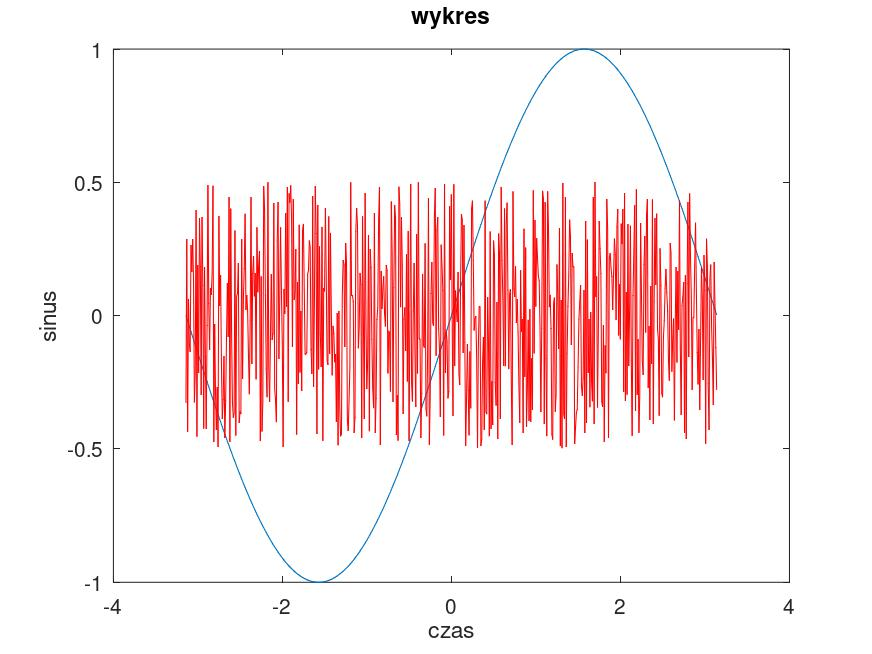
\includegraphics[width=\textwidth]{laboratorium_0_1-1.jpg}
\end{figure}
\begin{figure}[!ht]
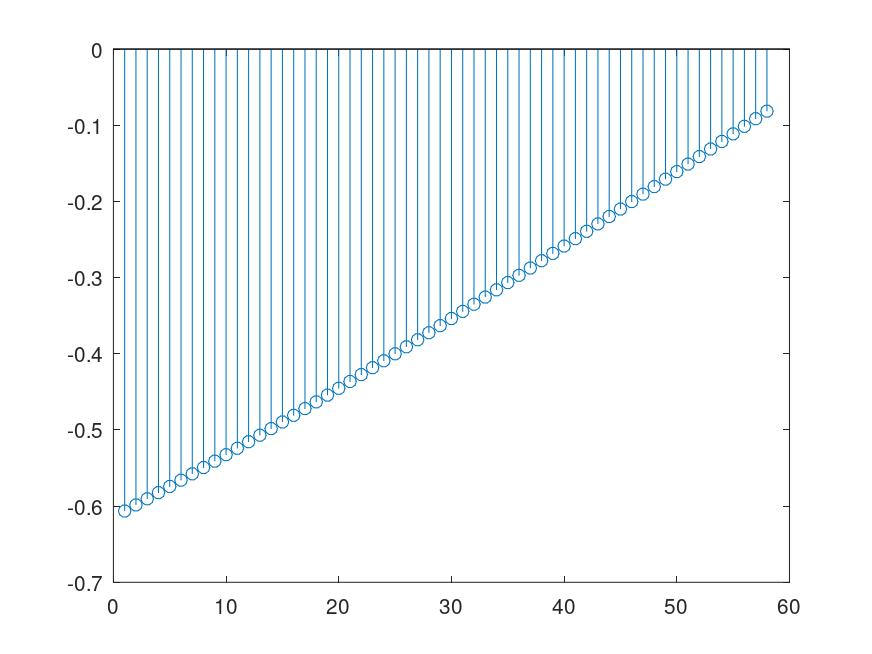
\includegraphics[width=\textwidth]{laboratorium_0_1-2.jpg}
\end{figure}
\begin{figure}[!ht]
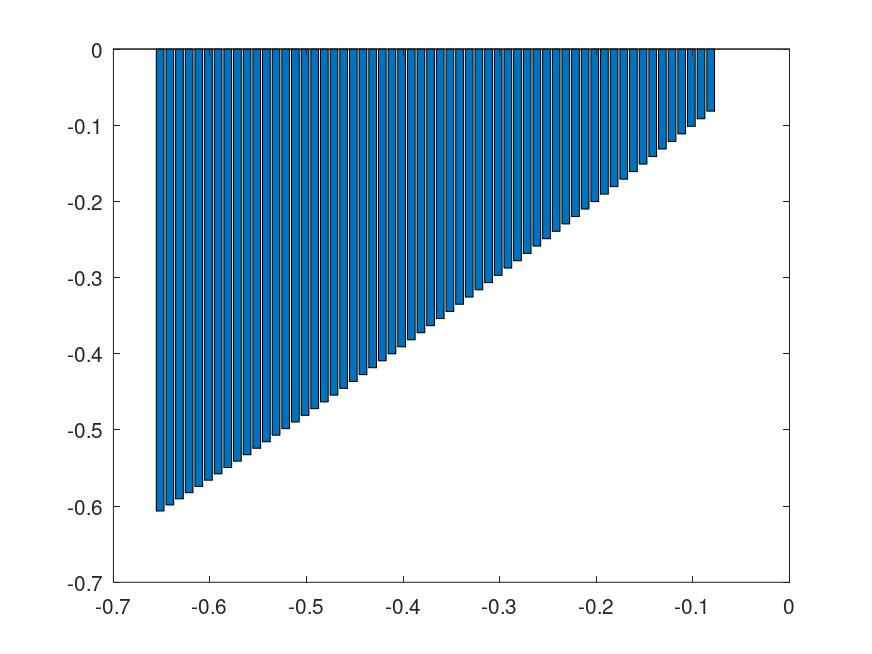
\includegraphics[width=\textwidth]{laboratorium_0_1-3.jpg}
\end{figure}
\begin{figure}[!ht]
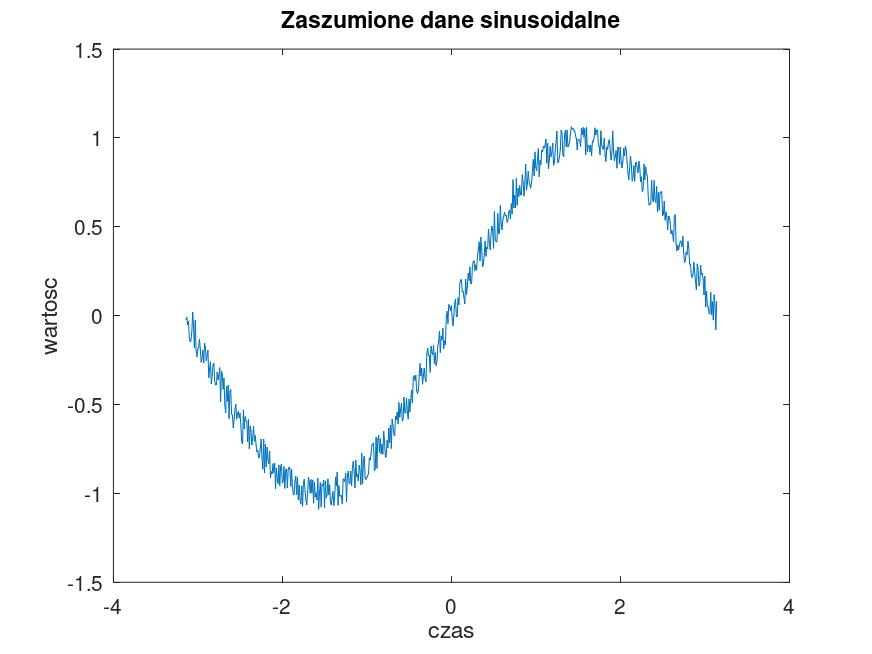
\includegraphics[width=\textwidth]{laboratorium_0_1-4.jpg}
\end{figure}


\phantomsection
\addcontentsline{toc}{section}{2.4.	Dane obrazowe}
\subsection*{2.4.	Dane obrazowe}



Matlab akceptuje (w sensie czytania i zapisu) obrazy w bardzo wielu
formatach (jpg, gif, bmp, png, itd.) ale ich wewnetrzna reprezentacja
jest zawsze taka sama.

\begin{lstlisting}
pkg load image

ImCol = uint8(zeros(128, 128, 3));
ImGray = uint8(zeros(128, 128));

% Typowa sekwencja wczytania, przetwarzania, wyswietlania i zapisu obrazu:
Im = imread('obraz.bmp');
figure(5); imshow(Im); % wyswietlenie wczytanego obrazu
ImZ = double(Im); % zamiana na postac zmiennoprzecinkowa...
ImZ = 255 - ImZ; % negatyw
figure(6); imshow(ImZ/255); % dlaczego dzielimy przez 255?
ImNew = uint8(ImZ); % powrot do reprezentacji bajtowej
imwrite(ImNew,'obraz_nowy.jpg'); % zapis do foldera
\end{lstlisting}
\begin{figure}[!ht]
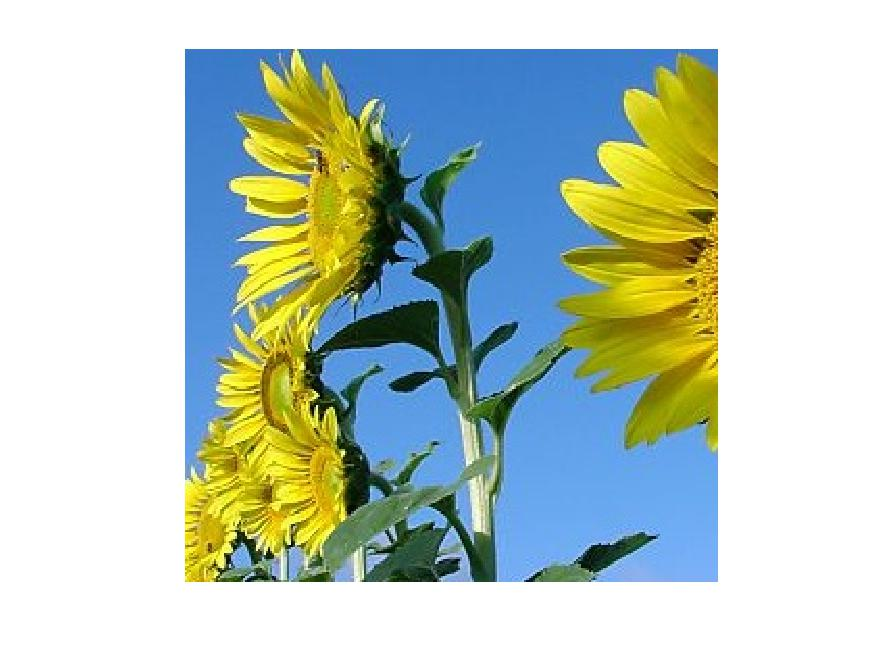
\includegraphics[width=\textwidth]{laboratorium_0_1-5.jpg}
\end{figure}
\begin{figure}[!ht]
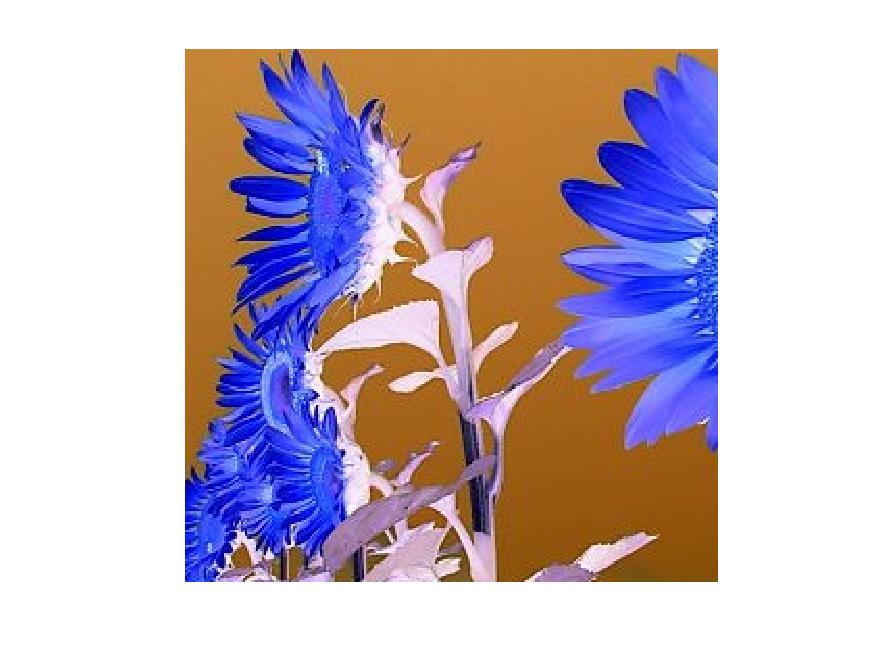
\includegraphics[width=\textwidth]{laboratorium_0_1-6.jpg}
\end{figure}


\phantomsection
\addcontentsline{toc}{section}{2.5.	Animacje (tworzenie, odczyt i zapis)}
\subsection*{2.5.	Animacje (tworzenie, odczyt i zapis)}



Typowa sekwencja odczytu i zapisu pliku video

\begin{lstlisting}
% Nie zaimplementowanie w Octave
%v = VideoReader('film_01.avi');
%v2 = VideoWriter('film_01','MPEG-4');
%open(v2);
%while hasFrame(v)
%    klatka = readFrame(v);
%    % ewentualne przetworzenie klatki
%    klatka1 = imresize(klatka,0.5);
%    writeVideo(v2,klatka1)  ;
%end
%close(v2);
\end{lstlisting}


\phantomsection
\addcontentsline{toc}{section}{2.6 FUNKCJE}
\subsection*{2.6 FUNKCJE}



Przyklady uzycia funkcji

\begin{lstlisting}
function  a = dodaj(b,c)
    a = b+c;
endfunction

b = 25; c = 75;
a = dodaj(b,c)
b1 = 4.567; c1 = 1.017 + 1i*0.589;
a1 = dodaj(b1,c1)
\end{lstlisting}
\begin{lstlisting}[language={},xleftmargin=5pt,frame=none]
a = 100
a1 =  5.5840 + 0.5890i

\end{lstlisting}


\phantomsection
\addcontentsline{toc}{section}{Typowy koniec skryptu}
\subsection*{Typowy koniec skryptu}

\begin{lstlisting}
% clear all; % usuniecie wszystkich zmiennych
% close all; % zamkniecie wszystkich wykresow
% clc % zresetowanie okna komend
\end{lstlisting}


\end{document}
